% !TEX program = pdflatex
\documentclass{article}
\usepackage[colorlinks=true,urlcolor=blue,citecolor=blue,linkcolor=blue]{hyperref} 

\usepackage{amsmath}
\usepackage{multirow}
\usepackage[linesnumbered, ruled, vlined]{algorithm2e}
\usepackage{graphicx}% Include figure files
\usepackage{subcaption}
\usepackage{tabularx}
\usepackage{listings}
\usepackage{marvosym}
\usepackage{amsthm}
\usepackage{cancel}
\usepackage{tikz}
\usepackage[mode=buildnew]{standalone}
\theoremstyle{definition}
\newtheorem{definition}{Definition}[section]
\newtheorem{theorem}{Theorem}[section]
\newtheorem{corollary}{Corollary}[section]
%\usepackage[linesnumbered, ruled, vlined, algo2e]{algorithm2e}
\lstset{
    basicstyle=\ttfamily\small,
    numberstyle=\scriptsize,
    % numbers=left,
    backgroundcolor=\color{white},
    %backgroundcolor=\color{white},
    %frame=single,
    xleftmargin=2em,
    tabsize=2,
    rulecolor=\color{black},
    %title=\lstname,
    escapeinside={(*}{*)},
    breaklines=true,
    %breakatwhitespace=true,
    %framextopmargin=2pt,
    %framexbottommargin=2pt,
    frame=bt,
    extendedchars=true,
    inputencoding=utf8,
    columns=fullflexible,
    %escapeinside={(*@}{@*)},
}

% the color of power ragers
\newcommand{\blue}[1]{[{\bf  \color{blue}{JG: #1}}]}
\newcommand{\Eq}[1]{Eq.~(\ref{#1})}
\newcommand{\Fig}[1]{Fig.~\ref{#1}}
\newcommand{\ra}[1]{\renewcommand{\arraystretch}{#1}}
\newcommand{\pdv}[2]{{\frac{\partial#1}{\partial#2}}}

\title{Quantum simulation on a random tensor network}
\begin{document}
\maketitle

\section{Differentiating single step time evolution}
The $m$ site Rydberg Hamiltonian is
\begin{equation}
    H_{\rm Rydberg} = \sum_{i,j=1, i>j}^{m} \frac{C}{|r_i-r_j|^6}n_i n_j + \Omega(t)\sum_{i=1}^{m} \frac{1}{2}\sigma_i^x + \Delta(t)\sum_{i=1}^{m} n_i
\end{equation}

For simplicity, we consider the following general representation of a time-space dependent Hamiltonian with $k$ terms
\begin{equation}
    H = \sum_{k=1}^{K} c_k O_k
\end{equation}
where $c_k$ can be dependent on a set of parameters like locations $r_1, r_2, \ldots, r_m$, and pulses $\Omega(t)$ and $\Delta(t)$.

\subsection{The ODE version}
In each step of the ODE solver, it performs the following update
\begin{equation}
    |\psi'\rangle = (1 - iH \Delta t) |\psi\rangle
\end{equation}

We derive the backward rules for the gradients by inspecting the following equations
% \begin{align}
%     &\overline{p} \mathrel{+}= \overline{c_k} \frac{\partial c_k}{\partial p}
% \end{align}

\begin{equation}\label{eq:ad0}
    \begin{split}
    \overline{\mathcal{L}}\delta \mathcal{L} &= \overline{|\psi'\rangle} \circ \delta |\psi'\rangle\\
    &= \sum_k \overline{c_k} \delta c_k + \overline{|\psi\rangle}\circ\delta|\psi\rangle + \overline{\Delta t}\delta \Delta t
    \end{split}
\end{equation}

where $\circ$ is the Hadamard product applied on real numbers,
note a complex number in computer is composed of two real numbers.
The above euqations has a more elegant linear algebra version as the following.

\begin{equation}\label{eq:ad1}
    \begin{split}
    \overline{\mathcal{L}}\delta \mathcal{L} &= \overline{\langle\psi'|} \delta |\psi'\rangle\\
    &= \sum_k \overline{c_k} \delta c_k + \overline{\langle\psi|}\delta|\psi\rangle + \overline{\Delta t}\delta \Delta t
    \end{split}
\end{equation}
where we have used $\langle\psi|$ to represent the hermitian conjugate of $|\psi\rangle$.

\begin{equation}\label{eq:ad2}
    \delta|\psi'\rangle = -i\sum_k \delta c_k O_k \Delta t |\psi\rangle - i H \delta \Delta t |\psi\rangle + (1-iH\Delta t) \delta |\psi\rangle
\end{equation}

By observing \Eq{eq:ad1} and \Eq{eq:ad2}, one can see
\begin{align}
    \overline{\langle\psi|} &= \overline{\langle\psi'|}(1-iH\Delta t)\\
    \overline{c_k} &= \Re\left[-i\Delta t\overline{\langle\psi'|} O_k|\psi\rangle\right]\\
    \overline{\Delta t} &= \Re\left[-i\overline{\langle\psi'|} H|\psi\rangle\right]
\end{align}

After a step, a normalization procedure might be called on the wave functions,
this is trivial so that we do not discuss it at this stage.

\subsection{The \texttt{expmv} version}
To differentiate the time evolution directly, one can use the Taylor expansion
\begin{equation}
    \begin{split}
    |\psi'\rangle &= e^{-iHt}|\psi\rangle\\
    & = \sum_{n=0}^{\infty}\frac{(-it)^n H^n}{n!}|\psi\rangle
    \end{split}
\end{equation}

Similarly, we have
\begin{equation}
    \delta|\psi'\rangle = e^{-iHt}\delta|\psi\rangle + \sum_{n=0}^{\infty}\frac{(-it)^n \delta (H^n)}{n!}|\psi\rangle + \left(e^{-iH(t+\delta t)}-e^{-iH t}\right)|\psi\rangle
\end{equation}

\begin{align}
    \overline{\langle\psi|} &= \overline{\langle\psi|}e^{-iHt}\delta\\
    \overline{t} &= \overline{\langle\psi'|}-iHe^{-iHt}|\psi\rangle\\
    \overline{c_k} &= \sum_n \frac{(-it)^n}{n!}\sum_{p=0}^{n-1} \overline{\langle\psi'|}H^p O_k H^{n-p-1}|\psi\rangle
\end{align}

\section{How to differentiate an ODE solver}
\subsection{The adjoint state method (or neural ODE)}
Since the time evolution is reversible, one can reverse it by doing inverse time evolution (or the adjoint state method~\cite{Plessix2006,Chen2018}).

\begin{algorithm}
    %\setstretch{1.35}
    \SetKwInOut{Input}{input}
    \SetKwInOut{Output}{output}
    \SetKwComment{Comment}{$\#$\ }{}
    \SetAlgoLined
    \DontPrintSemicolon
    \SetKwProg{Fn}{function}{}{end}
    \Input{parameters $\theta$, initial time $t_0$, ending time $t_n$, final state $s_n$ and its adjoint $\overline{s_n}$}
    \Output{$\overline{s_0}$, $\overline{\theta}$}
        \Fn{\rm aug\_dynamics(($s$, $a$, -), $t$, $\theta$)}{$q=f(s, t, \theta)$ \Comment*[r]{the augmented dynamics} \textbf{return} ($q$, $-a^T\frac{\partial q}{\partial s}$, $-a^T\frac{\partial q}{\partial \theta}$)}
        $S_0$ = ($s_n$, $\overline{s_n}$, $0$) \Comment*[r]{initial state of the augmented dynamics}
        ($s_0$, $\overline{s_0}$, $\overline{\theta}$) = ODESolve(aug\_dynamics, $S_0$, $\theta$, $t_n$, $t_0$) \Comment*[r]{integrate the augmented dynamics in the reversed time}
    \caption{The continuous adjoint state method}\label{alg:adjointstate}
\end{algorithm}


\subsection{The treeverse algorithm (or optimal checkpointing)}

For the cases reversibility is not guarented, one can use treeverse algorithm~\cite{Griewank1992,TreeverseAlgorithm}.
Peter is a road maintainer.
He is assigned a job by his male willed employer to paint a one-way road to blue in the reversed order (do not ask me why!).
Lucky enough, Peter picked up some teleportation magics in Hogwarts.
In the following illustration, we represent the road as $N$ grids arranged in one dimension.

\centerline{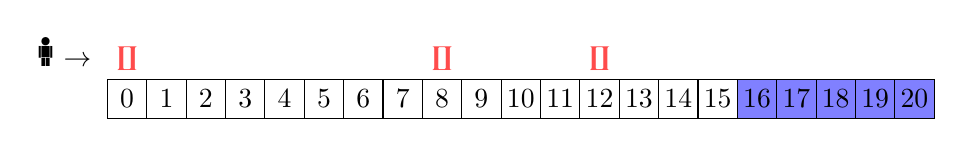
\begin{tikzpicture}
    \node at (-0.8, 0.6) () {{\Large \Gentsroom} $\rightarrow$};
    \node at (-0, 0.5) () {{\large \color{red!70}{\Gemini}}};
    \node at (4, 0.5) () {{\large \color{red!70}{\Gemini}}};
    \node at (6, 0.5) () {{\large \color{red!70}{\Gemini}}};
    \foreach \x in {0,...,20}
        \node[draw=black, minimum size=0.5cm, inner sep=0cm] at (0.5*\x, 0) () {\x};
    \foreach \x in {16,...,20}
        \node[draw=black, fill=blue!50, minimum size=0.5cm, inner sep=0cm] at (0.5*\x, 0) () {\x};
\end{tikzpicture}}

Peter can take the following actions.
\begin{enumerate}
    \item paint one block $s_i$ if he is in $i$-th block and $s_{i+1}$ is painted,
    \item move in one direction, i.e. $i\rightarrow i+1$,
    \item setup a teleportation gate (marked with red symbols) at where he locates.
    He can at most create $\delta \leq N$ gates at the same time.
    When this upper limit is reached, he must distroy an existing teleportation gate to create a new one.
    \item teleport himself to any existing teleportation gate.
\end{enumerate}

Given $N=10000$, $\delta=10$, can you please help Peter design a scheme so that he can drive the least?

The optimal solution is described by the binomial function $\eta(d, t) \equiv \frac{(d+t)!}{d!t!}$.
\begin{enumerate}
    \item In the first forward sweep, Peter uses teleportation gates to devide the road into $\delta$ segments of size $\eta(d, \tau-1), d=\delta,\delta-1,\ldots,1$ plus one extra grid. 
    Note $\sum_{d=0}^{\delta} \eta(d,\tau-1) = \eta(\delta,\tau)$.
    \item Sweep over the last block, use up the remaining checkpoints and paint the last grid. If Peter has paint all grids in a block, destroy the last checkpoint.
    \item In the $t$-th forward sweep of a block, Peter uses teleportation gates to devide the block into $d$ segments of size $\eta(k, \tau-t), k=d,d-1,\ldots,1$ plus one extra grid, where $d$ is equal to $\delta$ minus the number of checkpoints already used. 
\end{enumerate}


\begin{algorithm}
    %\setstretch{1.35}
    \SetAlgoLined
    \DontPrintSemicolon
    \SetKwProg{Fn}{function}{}{end}
    \SetKwInOut{Input}{input}
    \SetKwInOut{Output}{output}
    \SetKwComment{Comment}{$\#$\ }{}
    \Input{State cache $S=\{0:s_0\}$, the initial adjoint $\overline{s_n}\equiv \frac{\partial \mathcal{L}}{\partial s_n}$, the maximum number of checkpoints $\delta$, the number of scan $\tau$, the starting location of current block $\beta=0$, the end point of current block $\phi=n$, and the bisection point of current block $\sigma=0$}
    \Output{Back-propagated adjoint $\overline{s_0} \equiv \frac{\partial \mathcal{L}}{\partial s_0}$}
    \Fn{\rm treeverse($S$, $\overline{s_\phi}$, $\delta$, $\tau$, $\beta$, $\sigma$, $\phi$)}{
        \If{\rm $\sigma > \beta$}{
            $\delta = \delta - 1$\;
            $s = S[\beta]$   \Comment*[r]{load initial state $s_\beta$}
            \For{$j=\beta,\beta+1, ..., \sigma-1$}{
                $s_{j+1} = f_j(s_j)$ \Comment*[r]{compute $s_\sigma$}
            }
            $S[\sigma] = s_\sigma$
        }

         \#~let $\kappa$ be the division point, call the treeverse algorithm recursively\;
        \While{\rm $\tau>0$ {\bf and} $\kappa={\rm mid}(\delta, \tau, \sigma, \phi) < \phi$}{
            $\overline{s_{\kappa}}$ = treeverse($S$, $\overline{s_\phi}$, $\delta$, $\tau$, $\sigma$, $\kappa$, $\phi$)\;
            $\tau = \tau-1$\;
            $\phi = \kappa$
        }

        $\overline{s_\sigma} = \overline{f_\sigma}(\overline{s_{\sigma+1}}, s_\sigma)$\Comment*[r]{back propagate the gradient}
        \If{\rm $\sigma>\beta$}{
            remove($S[\sigma]$) \Comment*[r]{remove state $s_\sigma$ from cache}
        }
        {\bf return} $\overline{s_\sigma}$
    }
    \Fn{\rm mid($\delta$, $\tau$, $\sigma$, $\phi$) \hspace{7cm}\# choose the bisection point}{
        $\kappa = \lceil(\delta\sigma + \tau\phi)/(\tau+\delta)\rceil$\;
        \If{$\kappa \geq \phi$ {\bf and} $\delta > 0$}{
            $\kappa$ = max($\sigma+1$, $\phi-1$)
        }
    }
    \caption{The Treeverse algorithm}\label{alg:treeverse}
\end{algorithm}


\bibliographystyle{plain}
\bibliography{refs}
\end{document}
